\documentclass[aspectratio=169]{beamer}

\usetheme{metropolis}

\beamertemplatenavigationsymbolsempty

\usepackage{graphicx}
\usepackage{booktabs}
\usepackage{smartdiagram}

\usepackage{xcolor}
\usepackage{graphicx}
\usepackage{multicol}
\usepackage{wrapfig}

\graphicspath{ {images/} }
\usepackage[export]{adjustbox}

%----------------------------------------------------------------------------------------
%	TITLE PAGE
%----------------------------------------------------------------------------------------

\title{Managing configuration drifts in large computing infrastructures:
an experimental approach at CERN}

\author{ \vspace{20px}
    \textbf{Student}: \hspace{7px} Andrea Giardini \\
    \textbf{Supervisor}: Prof. Anna Ciampolini \\
    \textbf{Mentor}: \hspace{9px} Ben Dylan Jones \\}

\institute{University of Bologna}

\date{December 19, 2016}

\begin{document}

\begin{frame}
\titlepage
\end{frame}

\begin{frame}
\frametitle{Outline}
\vspace{10px}
\tableofcontents
\end{frame}

%------------------------------------------------
%	PRESENTATION SLIDES
%------------------------------------------------

%------------------------------------------------
\section{Introduction}
%------------------------------------------------

\subsection{CERN}
\begin{frame}
    \frametitle{CERN}
    \begin{minipage}[t]{0.95\textwidth}
        \begin{columns}
            \begin{column}{0.5\textwidth}
                \begin{itemize}
                    \item European Organization for Nuclear Research
                    \item Situated in the border between Switzerland and France
                    \item 21 Member states
                    \item Big challenges 
                \end{itemize}
            \end{column}
            \begin{column}{0.5\textwidth}
                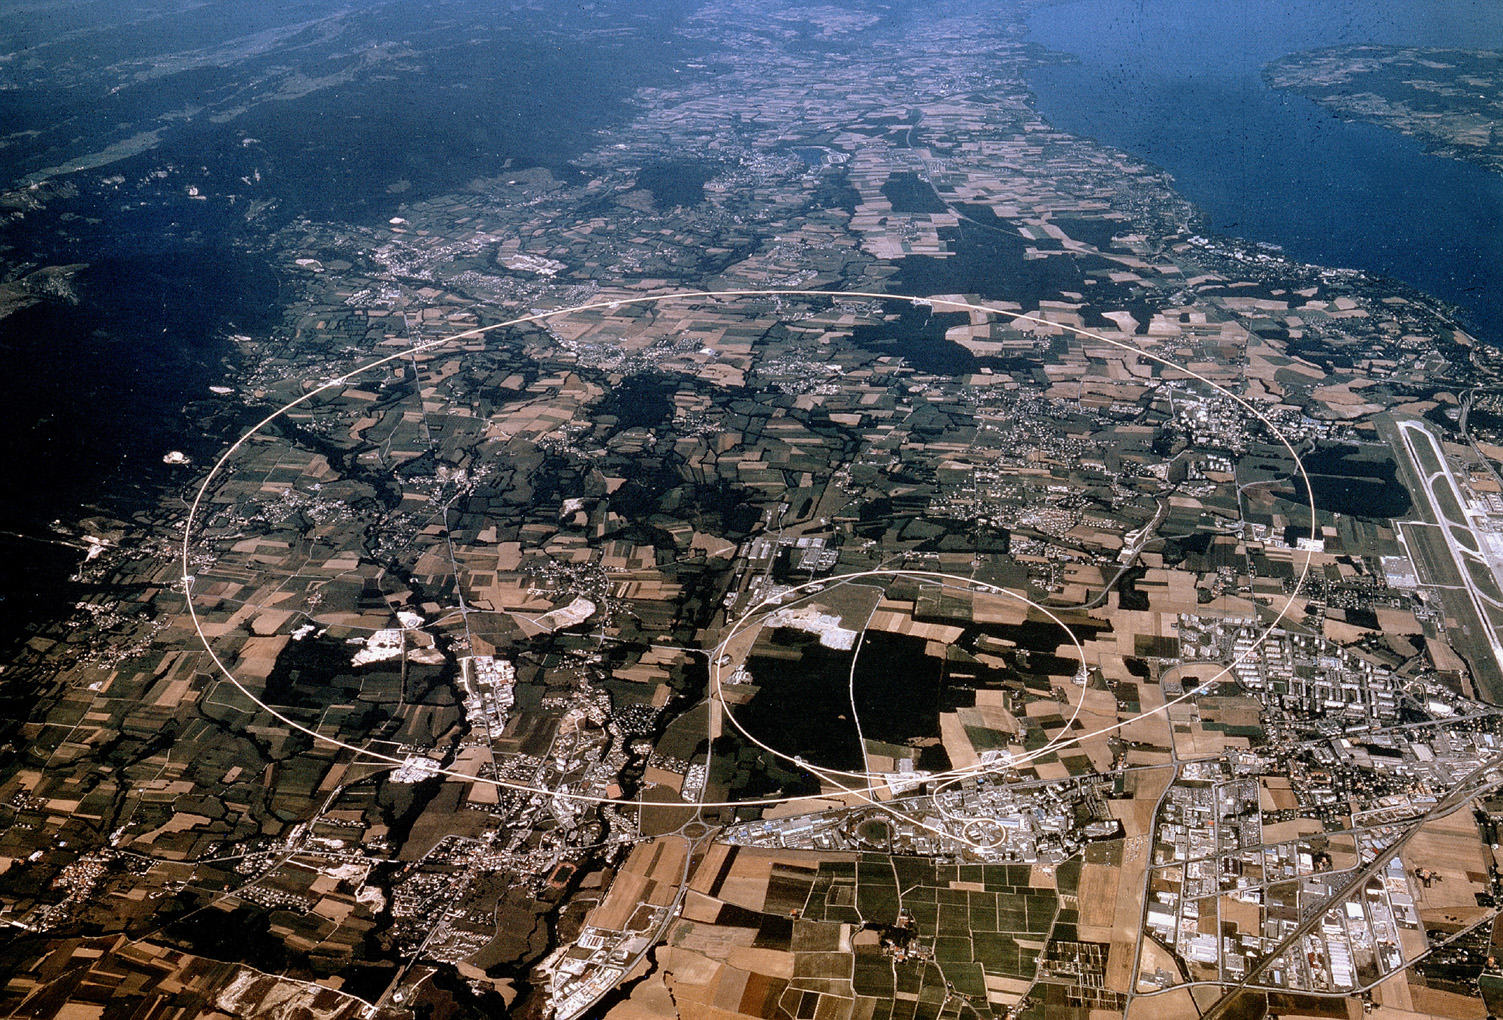
\includegraphics[width=1.1\textwidth]{CernMap.jpg}
            \end{column}
        \end{columns}
    \end{minipage}
\end{frame}

%------------------------------------------------

\begin{frame}
    \frametitle{Data Centres}
    \begin{minipage}[t]{0.95\textwidth}
        \begin{columns}[T]
            \begin{column}{0.5\textwidth}
                Two data centers:
                \begin{itemize}
                    \item Budapest
                    \item Geneva
                \end{itemize}
                Two dedicated links:
                \begin{itemize}
                    \item 2 x 100Gbps
                \end{itemize}
                \vspace{0.1in}
                The number of resources is growing year by year.
                As today:
                \begin{itemize}
                    \item 18k servers
                    \item 180PB on tape
                    \item 260PB on disk
                \end{itemize}
            \end{column}
            \begin{column}{0.5\textwidth}
                \vspace{0.5in}
                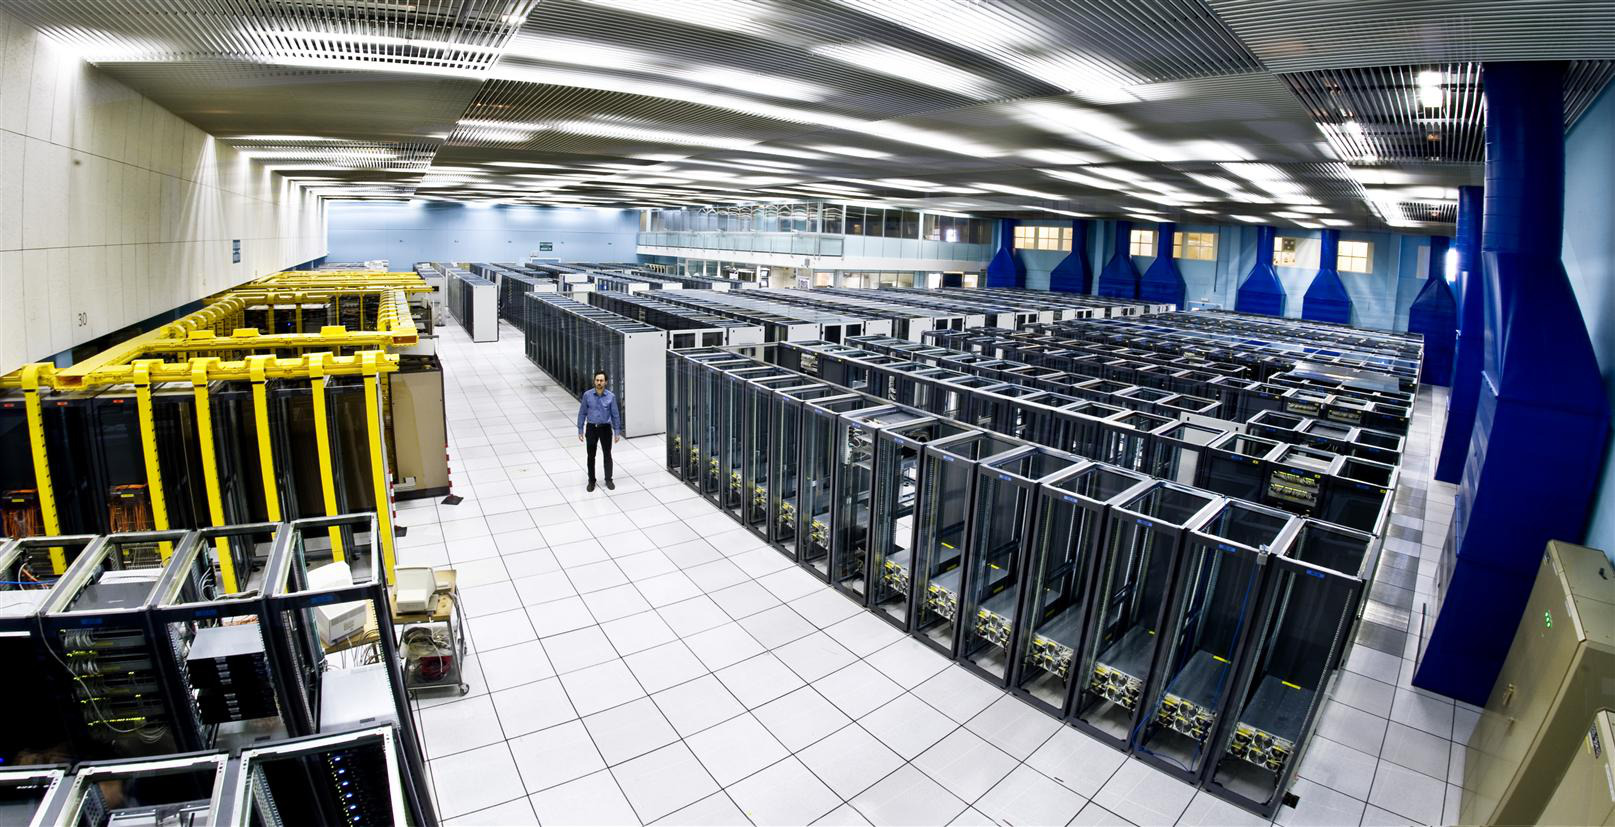
\includegraphics[width=1.1\textwidth]{DC_overview.png}
            \end{column}
        \end{columns}
    \end{minipage}
\end{frame}

%------------------------------------------------

\subsection{Configuration management}
\begin{frame}
    \frametitle{Going Agile}
    \begin{minipage}[t]{0.95\textwidth}
        \begin{columns}
            \begin{column}{0.8\textwidth}
                Requirements started to grow
                \begin{itemize}
                    \item Agile approach was needed
                \end{itemize}
                Since a few years we started using Openstack to deploy virtual
                machines for our users and Puppet to configure the services 
            \end{column}
            \begin{column}{0.2\textwidth}
                
\includegraphics[width=0.9\textwidth]{openstack-logo512.png}
            \end{column}
        \end{columns}
    \end{minipage}
    \vspace{\belowdisplayskip}
    \vspace{\belowdisplayskip}
    \begin{minipage}[t]{0.95\textwidth}
        \begin{center}
        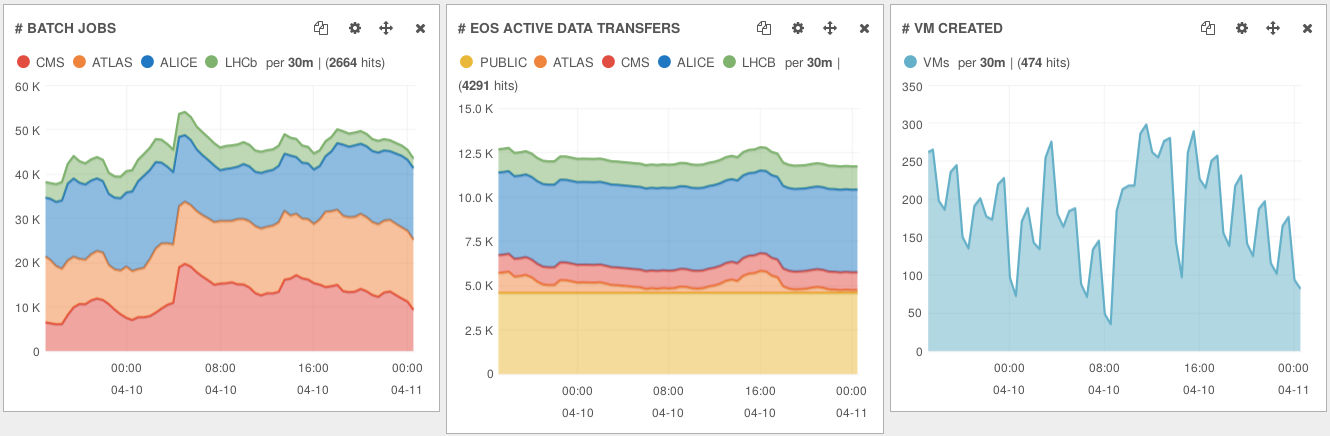
\includegraphics[width=0.83\textwidth]{Eos-CreatedVm.png}
    \end{center}
    \end{minipage}
\end{frame}

%------------------------------------------------

\begin{frame}
    \frametitle{Configuration Management with Puppet}
    \begin{minipage}[t]{0.95\textwidth}
        \begin{columns}
            \begin{column}{0.5\textwidth}
                Puppet is an open-source configuration management tool.
                It is designed to manage the configuration of Unix-like and Microsoft Windows systems declaratively. \\
                \begin{itemize}
                    \item Service configuration
                    \item Users/Groups management
                    \item Automates repetitive taks
                \end{itemize}
            \end{column}
            \begin{column}{0.5\textwidth}
                \vspace{-10px}
                
\includegraphics[width=1.1\textwidth]{puppet-labs-logo.png}
            \end{column}
        \end{columns}
    \end{minipage}
\end{frame}

%------------------------------------------------

\begin{frame}
    \frametitle{Problems}
    \begin{itemize}
        \item Multiple service managers
        \item Deployment interval
        \item Configuration and package drifting
    \end{itemize}
\end{frame}

%------------------------------------------------
\section{Package Inventory}
%------------------------------------------------

\begin{frame}
    \frametitle{Introduction}
    \vspace{10px}
    \begin{minipage}[t]{0.95\textwidth}
        Configuration drifts started to be a problem:
        \begin{itemize}
            \item Servers with outdated packages
            \item Difficult to spot
            \item Users forcing their servers not to update
        \end{itemize}
        It is not easy to keep all the configuration in sync and guarantee security
    \end{minipage}
    \vspace{\belowdisplayskip}
    \begin{minipage}[t]{0.95\textwidth}
        \begin{center}
            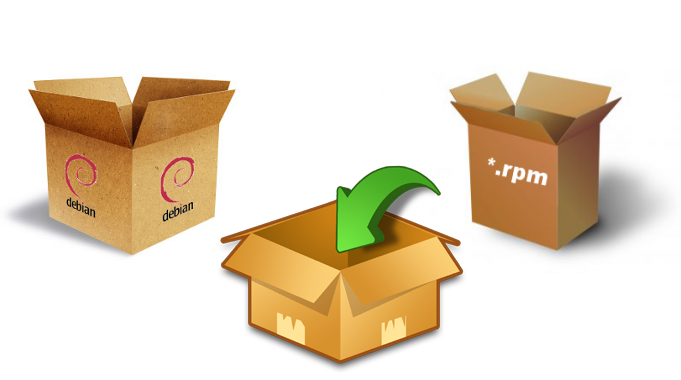
\includegraphics[width=0.5\textwidth]{package.png}
        \end{center}
    \end{minipage}
\end{frame}

%------------------------------------------------

\subsection{Project Structure}
\begin{frame}
    \frametitle{Project Structure}
    The configuration team needed a tool to query packages over a large
    number of hosts in a timely manner.

    Package Inventory is made by three components:
    \begin{itemize}
        \item Reporter
        \item Cli
        \item Elasticsearch Cluster
    \end{itemize}
\end{frame}

%------------------------------------------------

\begin{frame}
    \frametitle{Reporter}
\end{frame}

%------------------------------------------------

\begin{frame}
    \frametitle{Cli}
    \begin{itemize}
        \item Possibility to compare clusters of machines
        \item Package history
    \end{itemize}
\end{frame}

%------------------------------------------------

\subsection{Results}
\begin{frame}
    \frametitle{Results}
    \begin{itemize}
        \item Installed in more than \textbf{55 hundreds of servers}
        \item Spotted over \textbf{two hundreds of servers} out of sync
        \item Used extensively to monitor the deployment of security updates
        \item Debugging performance issues
    \end{itemize}
\end{frame}

%------------------------------------------------
\section{Continuous Integration}
%------------------------------------------------

\begin{frame}
    \frametitle{Introduction}

    Automated way to ship configuration changes to production
\end{frame}

%------------------------------------------------

\subsection{Project Structure}
\begin{frame}
    \frametitle{Project Structure}
    \begin{minipage}[t]{0.95\textwidth}
        \begin{columns}
            \begin{column}{0.5\textwidth}
            Implementation of a Continuous Integration platform using Jenkins
            \begin{itemize}
                \item Open source software
                \item Highly customizable
                \item Active community
            \end{itemize}
            blabla 
            \end{column}
            \begin{column}{0.5\textwidth}
                \vspace{-10px}
                
\includegraphics[width=1.1\textwidth]{jenkins-logo.png}
            \end{column}
        \end{columns}
    \end{minipage}
\end{frame}

%------------------------------------------------

\begin{frame}
    \frametitle{Manual CRM process}
    \smartdiagramset{sequence item border color=black,
        sequence item border size=1pt,
        sequence item font size=\small\sffamily,
        set color list={red!50,red!50,red!50}
    }
    \smartdiagram[sequence diagram]
        {Push the change to custom Git branch,
        Open JIRA issue describing the change,
        Open merge request on Gitlab to QA}
    \vspace{20px}
    \smartdiagram[sequence diagram]
        {Approve merge request on Gitlab,
        Open merge request on Gitlab to master,
        Approve merge request on Gitlab}
\end{frame}

%------------------------------------------------

\begin{frame}
    \frametitle{Automated CRM Process}
    \smartdiagramset{sequence item border color=black,
        sequence item border size=1pt,
        sequence item font size=\small\sffamily,
        set color list={red!50,red!50,orange!50}
    }
    \smartdiagram[sequence diagram]
        {Push the change to custom Git branch,
        Open JIRA issue describing the change,
        Open merge request on Gitlab to QA}
    \vspace{20px}
    \smartdiagramset{set color list={red!50,red!50,red!50}}
    \smartdiagram[sequence diagram]
        {Approve merge request on Gitlab,
        Open merge request on Gitlab to master,
        Approve merge request on Gitlab}
\end{frame}

%------------------------------------------------

\begin{frame}
    \frametitle{Automated CRM Process}
    \smartdiagramset{sequence item border color=black,
        sequence item border size=1pt,
        sequence item font size=\small\sffamily,
        set color list={red!50,red!50,orange!50,green!50}
    }
    \smartdiagram[sequence diagram]
        {Push the change to custom Git branch,
        Open JIRA issue describing the change,
        Open merge request on Gitlab to QA,
        Run automated tests on Jenkins}
    \vspace{20px}
    \smartdiagramset{set color list={red!50,red!50,red!50}}
    \smartdiagram[sequence diagram]
        {Approve merge request on Gitlab,
        Open merge request on Gitlab to master,
        Approve merge request on Gitlab}
\end{frame}

%------------------------------------------------

\begin{frame}
    \frametitle{Automated CRM Process}
    \smartdiagramset{sequence item border color=black,
        sequence item border size=1pt,
        sequence item font size=\small\sffamily,
        set color list={red!50,red!50,orange!50,green!50}
    }
    \smartdiagram[sequence diagram]
        {Push the change to custom Git branch,
        Open JIRA issue describing the change,
        Open merge request on Gitlab to QA,
        Run automated tests on Jenkins}
    \vspace{20px}
    \smartdiagramset{set color list={orange!50,red!50,red!50}}
    \smartdiagram[sequence diagram]
        {Approve merge request on Gitlab,
        Open merge request on Gitlab to master,
        Approve merge request on Gitlab}
\end{frame}

%------------------------------------------------

\begin{frame}
    \frametitle{Automated CRM Process}
    \smartdiagramset{sequence item border color=black,
        sequence item border size=1pt,
        sequence item font size=\small\sffamily,
        set color list={red!50,red!50,orange!50,green!50}
    }
    \smartdiagram[sequence diagram]
        {Push the change to custom Git branch,
        Open JIRA issue describing the change,
        Open merge request on Gitlab to QA,
        Run automated tests on Jenkins}
    \vspace{20px}
    \smartdiagramset{set color list={orange!50,orange!50,red!50}}
    \smartdiagram[sequence diagram]
        {Approve merge request on Gitlab,
        Open merge request on Gitlab to master,
        Approve merge request on Gitlab}
\end{frame}

%------------------------------------------------

\begin{frame}
    \frametitle{Automated CRM Process}
    \smartdiagramset{sequence item border color=black,
        sequence item border size=1pt,
        sequence item font size=\small\sffamily,
        set color list={red!50,red!50,orange!50,green!50}
    }
    \smartdiagram[sequence diagram]
        {Push the change to custom Git branch,
        Open JIRA issue describing the change,
        Open merge request on Gitlab to QA,
        Run automated tests on Jenkins}
    \vspace{20px}
    \smartdiagramset{set color list={orange!50,orange!50,green!50}}
    \smartdiagram[sequence diagram]
        {Approve merge request on Gitlab,
        Open merge request on Gitlab to master,
        Run automated tests on Jenkins}
\end{frame}

%------------------------------------------------

\begin{frame}
    \frametitle{Automated CRM Process}
    \smartdiagramset{sequence item border color=black,
        sequence item border size=1pt,
        sequence item font size=\small\sffamily,
        set color list={red!50,red!50,orange!50,green!50}
    }
    \smartdiagram[sequence diagram]
        {Push the change to custom Git branch,
        Open JIRA issue describing the change,
        Open merge request on Gitlab to QA,
        Run automated tests on Jenkins}
    \vspace{20px}
    \smartdiagramset{set color list={orange!50,orange!50,green!50,orange!50}}
    \smartdiagram[sequence diagram]
        {Approve merge request on Gitlab,
        Open merge request on Gitlab to master,
        Run automated tests on Jenkins,
        Approve merge request on Gitlab}
\end{frame}

%------------------------------------------------

\subsection{Results}
\begin{frame}
    \frametitle{Results}
    \begin{itemize}
        \item Extremely customizable infrastructure
        \begin{itemize}
            \item Users can define their tests
            \item Service managers specify how the test server needs to be built
            \item Tests can be re-triggered with a comment on JIRA or pushing new commits
        \end{itemize}
        \item Every service manager is responsible for its Puppet module
        \item Procedure completely automated
        \item No need for users to learn how to use Jenkins
    \end{itemize}
\end{frame}

%------------------------------------------------
\section{Conclusions}
%------------------------------------------------

\begin{frame}
    \frametitle{Conclusions}
\end{frame}

\end{document}
